\documentclass[10pt,aspectratio=169]{beamer}
%\documentclass[10pt]{beamer}

\usetheme[sectionpage=none] % TODO solve the arithmetic error problem later (on section pages)
  {metropolis}
\usepackage{appendixnumberbeamer}

\usepackage{verbatim}

% strikethrough
% - normalem: do not redefine emph to do underline
\usepackage[normalem]{ulem}

% bold math
\usepackage{bm}

\usepackage{xcolor,soul}
\definecolor{lightblue}{rgb}{.90,.95,1}
\definecolor{lightred}{rgb}{1,.80,.80}
\definecolor{lightgreen}{rgb}{.80,1.,.80}
%\definecolor{lightred}{red!40}
\sethlcolor{lightblue}

\definecolor{rosenpass-pink}{RGB}{247, 4, 132}
\definecolor{rosenpass-orange}{RGB}{255, 166, 48}
\definecolor{rosenpass-gray}{RGB}{64, 63, 76}
\definecolor{rosenpass-lightblue}{RGB}{211, 243, 238}
\definecolor{rosenpass-blue}{RGB}{114, 161, 229}

\setbeamercolor{progress bar}{fg=rosenpass-pink,bg=blue}
\setbeamercolor{title separator}{fg=rosenpass-pink,bg=blue}


\renewcommand<>{\hl}[1]{\only#2{\beameroriginal{\hl}}{#1}}
\usepackage[beamer]{hf-tikz}
\usetikzlibrary{arrows.meta}
\tikzset{
	>=Latex[round]
}

\urlstyle{same}

% https://tex.stackexchange.com/questions/41683/why-is-it-that-coloring-in-soul-in-beamer-is-not-visible
\makeatletter
\newcommand\SoulColor{%
  \let\set@color\beamerorig@set@color
  \let\reset@color\beamerorig@reset@color}
  \makeatother
  \SoulColor

\setlength{\fboxsep}{0pt}
\newcommand{\mathcolorbox}[2]{\colorbox{#1}{$\displaystyle #2$}}
\newcommand{\ah}[1]{\colorbox{lightblue}{$\displaystyle #1$}}
\newcommand{\bh}[1]{\colorbox{lightred}{$\displaystyle #1$}}
\newcommand{\ch}[1]{\colorbox{lightgreen}{$\displaystyle #1$}}
\newcommand{\hlfancy}[2]{\sethlcolor{#1}\hl{#2}}

\setbeamercolor{frametitle}{parent=subtitle}
% `title separator` is the one on the title page
% `progress bar in head/foot` is the line on each frame
\setbeamercolor{progress bar in head/foot}{bg=normal text.bg,fg=normal text.bg}

\usepackage{appendixnumberbeamer}

\usepackage{booktabs}
\usepackage[scale=2]{ccicons}
\usepackage{fontawesome}

\usepackage{pgfplots}
\usepgfplotslibrary{dateplot}

%% tikzit
%\usepackage{tikzit}
%\input{blipp.tikzstyles}
%\usetikzlibrary{trees}
%\usetikzlibrary{tikzmark}
%\usetikzlibrary{arrows.meta}

\usepackage{xspace}
\newcommand{\themename}{\textbf{\textsc{metropolis}}\xspace}


\usepackage{stackengine}
\usepackage{amsmath}
\usepackage{amsfonts}
\usepackage{amssymb}
\usepackage{amsthm}
\usepackage{tikz}
\usepackage{xcolor}
\usepackage{environ}
\usepackage{array}
\usepackage[
  n,advantage,operators,sets,adversary,landau,
  probability,
  notions,logic,ff,mm,primitives,events,complexity,asymptotics
  %keys
  ]{cryptocode}
\usetikzlibrary{positioning,shapes,arrows,matrix, calc,external,fit,decorations.pathreplacing,arrows.meta,patterns,tikzmark}


\usepackage{mathtools}
\usepackage{comment}
\excludecomment{commentEnv}
\usepackage{array}
\newcolumntype{C}[1]{>{\centering\let\newline\\\arraybackslash\hspace{0pt}}m{#1}}


\def\makeuppercase#1{
\expandafter\newcommand\csname cal#1\endcsname{\mathcal{#1}}
\expandafter\newcommand\csname adv#1\endcsname{\mathcal{#1}}
\expandafter\newcommand\csname frak#1\endcsname{\mathfrak{#1}}
\expandafter\newcommand\csname bb#1\endcsname{\mathbb{#1}}
\expandafter\newcommand\csname bf#1\endcsname{\textbf{#1}}
}




\def\makelowercase#1{
\expandafter\newcommand\csname frak#1\endcsname{\mathfrak{#1}}
\expandafter\newcommand\csname bf#1\endcsname{\textbf{#1}}
}

\newcounter{char}
\setcounter{char}{1}

\loop
	\edef\letter{\alph{char}}
	\edef\Letter{\Alph{char}}
	\expandafter\makelowercase\letter
	\expandafter\makeuppercase\Letter
	\stepcounter{char}
	\unless\ifnum\thechar>26
\repeat


\newcommand{\quotes}[1]{``#1''}
\newcommand{\filename}[1]{\texttt{#1}}
\newcommand{\cryptoverif}{Crypto\-Verif}
\newcommand{\cv}{\cryptoverif}
\newcommand{\bottom}{\ensuremath{\perp}}


%\usepackage{pgfpages}
%\setbeameroption{show notes on second screen=right} 

\usepackage{multicol}
\usepackage{qrcode}



%% msc message diagrams
%\usepackage{msc5}
%\newcommand{\laction}[2]{$\begin{array}{c}\mbox{\textrm{#1}}\\#2\end{array}$}
%\newcommand{\poormanshead}[1]{\textcolor{darkgray}{#1}}
%\newcommand{\poormansline}[2]{\textcolor{gray}{\phantom{-- }\texttt{-- -- -- -- -- -- -- --\phantom{ --}}}\poormanshead{#1}\textcolor{gray}{\texttt{\phantom{-- }#2}}}


\definecolor{light-gray}{gray}{0.5}
% https://gamedev.stackexchange.com/questions/133078/what-colors-to-choose-for-colorblind-people
\definecolor{keyOne}{rgb}{.9,.6,0} % orange
\definecolor{keyTwo}{rgb}{.35,.7,.9} % sky blue
\definecolor{keyThree}{rgb}{0,.6,.5} % bluish green
\definecolor{keyFour}{rgb}{.8,.4,0} % vermilion
%\definecolor{keyFour}{rgb}{.8,.6,.7} % reddish purple
%\definecolor{keyFour}{rgb}{0,.45,.7} % blue


\newcommand{\screenshotframe}[2]{%
\begin{frame}{#1}
  \vfill
  \begin{center}
    \includegraphics[width=.95\textwidth,height=.95\textheight,keepaspectratio]{#2}
  \end{center}
  \vfill
\end{frame}
}

\usepackage{listings}
\lstdefinelanguage{cryptoverif}
{morekeywords={collision, const, crypto, define, defined, do, else, end, equation, equiv,
event, event_abort, expand, find, forall, foreach, fun, get, implementation, in,
if, inj, insert, length, let, letfun, max, maxlength, newOracle, orfind, otheruses,
param, proba, public_vars, process, proof, query, return, secret, secret1, set, suchthat, success, simplify, then,
table, time, type},
otherkeywords={<-, <-R, &&},
sensitive=true,
morecomment=[s]{(*}{*)},
morestring=[b]",
}
\lstdefinelanguage{cvoutput}
{morekeywords={},
otherkeywords={},
sensitive=true,
morecomment=[s]{(*}{*)},
morestring=[b]",
}
\lstset{
  language=cvoutput,
  basicstyle=\ttfamily,
  commentstyle=\color{black!55},
  keywordstyle=\bfseries\color{green!40!black}
}
\lstset{
  language=cryptoverif,
  basicstyle=\ttfamily,
  commentstyle=\color{black!55},
  keywordstyle=\bfseries\color{green!40!black}
}

\usepackage{bbding}
\newcommand*\itemtick{\item[\Checkmark]}
\newcommand*\itemfail{\item[\XSolidBrush]}

\title{%
  Rosenpass
}
\subtitle{%
  Securing \& Deploying Post-Quantum WireGuard
}
\author{\textbf{Karolin Varner}, with Benjamin Lipp, Wanja Zaeske, Lisa Schmidt}
\institute{RWPQC23 | \url{https://rosenpass.eu/whitepaper.pdf}}
\titlegraphic{\hfill
\includegraphics[height=2.5cm]{RosenPass-Logo.pdf}}

\usepackage[autostyle]{csquotes}

\begin{document}

\date{26 March 2023}

\maketitle

% 

\begin{frame}{Structure of the talk}
\begin{itemize}
  \item Post-quantum WireGuard\footnote{
	  Andreas Hülsing, Kai-Chun Ning, Peter Schwabe, Florian Weber, and Philip R. Zimmermann. “Post-quantum WireGuard”. In: 42nd IEEE Symposium on Security and Privacy, SP 2021, San Francisco, CA, USA, 24-27 May 2021. Full version: https://eprint.iacr.org/2020/379
	}: How to build an interactive key exchange from KEMs
  \item Contribution: State Disruption Attacks \& cookies as a defense
  \item Contribution: Symbolic analysis of the Rosenpass protocol
  \item Contribution: Noise-like specification
  \item Contribution: New hashing \& domain separation scheme
  \item Contribution: Reference implementation – Securing WireGuard in practice
\end{itemize}
\end{frame}

\begin{frame}{Post-quantum WireGuard: Three encapsulations}
\tikzset{shorten > = 1pt,shorten < = 1pt}
\begin{columns}

\begin{column}{.30\textwidth}
\begin{tikzpicture}
	 \draw (-1,0) node[above](initiator){Initiator\strut} --
		coordinate[pos=.2](spkr-y)
		coordinate[pos=.6](sctr-y)
		coordinate[pos=.76](ack-y)+(0,-5);
	  \draw (1,0) node[above](responder){Responder\strut}-- +(0,-5);


		\draw[<-](spkr-y-|initiator) -- node[above]{spkr} (spkr-y-|responder);
		\draw[->](sctr-y-|initiator) -- node[above] {sctr} (sctr-y-|responder);
		\draw[<-](ack-y-|initiator) -- node[above] {(ack)} (ack-y-|responder);

\end{tikzpicture}
Responder Auth
\end{column}

\begin{column}{.30\textwidth}
\begin{tikzpicture}
	 \draw (-1,0) node[above](initiator){Initiator\strut} --
		coordinate[pos=.2](spki-y)
		coordinate[pos=.6](Hspki-y)
		coordinate[pos=.76] (scti-y)
		coordinate[pos=.92](ack-y)+(0,-5);
	 \draw (1,0) node[above](responder){Responder\strut}-- +(0,-5);

	 \draw[->](spki-y-|initiator) -- node[above]{spki} (spki-y-|responder);
	 \draw[->](Hspki-y-|initiator) -- node[above] {H(spki)} (Hspki-y-|responder);

	  \draw[<-](scti-y-|initiator) -- node[above]{scti} (scti-y-|responder);

	 \draw[->](ack-y-|initiator) -- node[above] {(ack)} (ack-y-|responder);

\end{tikzpicture}
Initiator Auth
\end{column}

\begin{column}{.30\textwidth}
\begin{tikzpicture}
	 \draw (-1,0) node[above](initiator){Initiator\strut} --
		coordinate[pos=.6](epki-y)
		coordinate[pos=.76] (ecti-y)
		coordinate[pos=.92](ack-y)+(0,-5);
	 \draw (1,0) node[above](responder){Responder\strut}-- +(0,-5);

	 \draw[->](epki-y-|initiator) -- node[above]{epki} (epki-y-|responder);
	 \draw[<-](ecti-y-|initiator) -- node[above]{ecti} (ecti-y-|responder);
	 \draw[->](ack-y-|initiator) -- node[above] {(ack)} (ack-y-|responder);

\end{tikzpicture}
Forward secrecy
\end{column}

\end{columns}
\end{frame}

\begin{frame}{Combining the three encapsulations in one protocol}

\begin{tikzpicture}[shorten > = 1pt,shorten < = 1pt]
	\draw (-3,0) node[above](initiator){Initiator\strut} -- coordinate[pos=.2](spki-y)
	coordinate[pos=.35](spkr-y)
	coordinate[pos=.6](epki-y)
	coordinate[pos=.75](scti-y)
	coordinate[pos=.9](ack-y)+(0,-5);
	\draw (3,0) node[above](responder){Responder\strut}-- +(0,-5);

	 \draw[->](spki-y-|initiator) -- node[above] {spki} (spki-y-|responder);
	 \draw[<-](spkr-y-|initiator) -- node[above] {spkr} (spkr-y-|responder);
	 \draw[->](epki-y-|initiator) -- node[above] {epki, sctr, H(spki)} (epki-y-|responder);
	 \draw[<-](scti-y-|initiator) -- node[above] {scti,ecti} (scti-y-|responder);
	  \draw[->](ack-y-|initiator) -- node[above] {(ack)} (ack-y-|responder);

\end{tikzpicture}

  Note that the initiator is not authenticated until they send \enquote{(ack)}.

\end{frame}

\begin{frame}{The Rosenpass protocol}
  \includegraphics[height=.9\textheight]{rosenpass-whitepaper-key-exchange-protocol}
\end{frame}

\begin{frame}{CVE-2021-46873 – DOS against WireGuard through NTP}
\begin{itemize}
  \item The replay protection in classic WireGuard assumes a monotonic counter
  \item But the system time is attacker controlled because NTP is insecure
  \item This generates a kill packet that abuses replay protection and renders the initiator's key-pair useless
  \item Attack is possible in the real world!
  \item Similar attack in post-quantum WireGuard is worse since InitHello is unauthenticated
  \item Solution: Biscuits
\end{itemize}
\end{frame}

\begin{frame}{Security analysis of rosenpass}
  \begin{itemize}
	\item CryptoVerif in progress
	\item Symbolic analysis using ProVerif
  \item Code is part of the software repository \& build system
  \item Symbolic analysis is fast (about five minutes), runs in parallel and is
  \end{itemize}
\end{frame}

\begin{frame}{ProVerif in technicolor}
  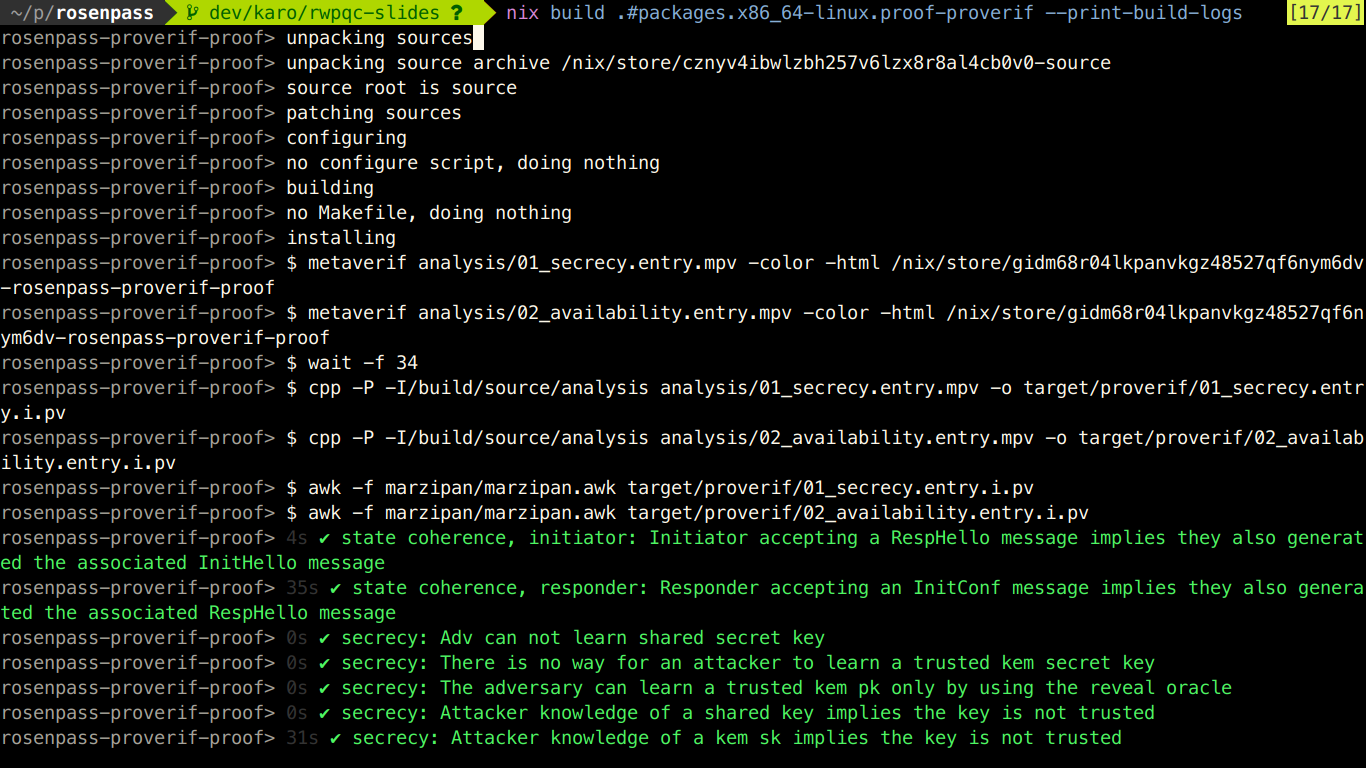
\includegraphics[height=.9\textheight]{assets/2023-03-20-symbolic-analysis-screenshot.png}
\end{frame}


\begin{frame}{Noise-like specification (easier for engineers)}
  \includegraphics[height=.9\textheight]{rosenpass-whitepaper-message-handling-code.pdf}
\end{frame}

\begin{frame}{New Hashing/Domain separation scheme}
  \includegraphics[height=.9\textheight]{rosenpass-whitepaper-hashing-tree.pdf}
\end{frame}

\begin{frame}{Reference implementation in rust, deploying post-quantum-secure WireGuard}
  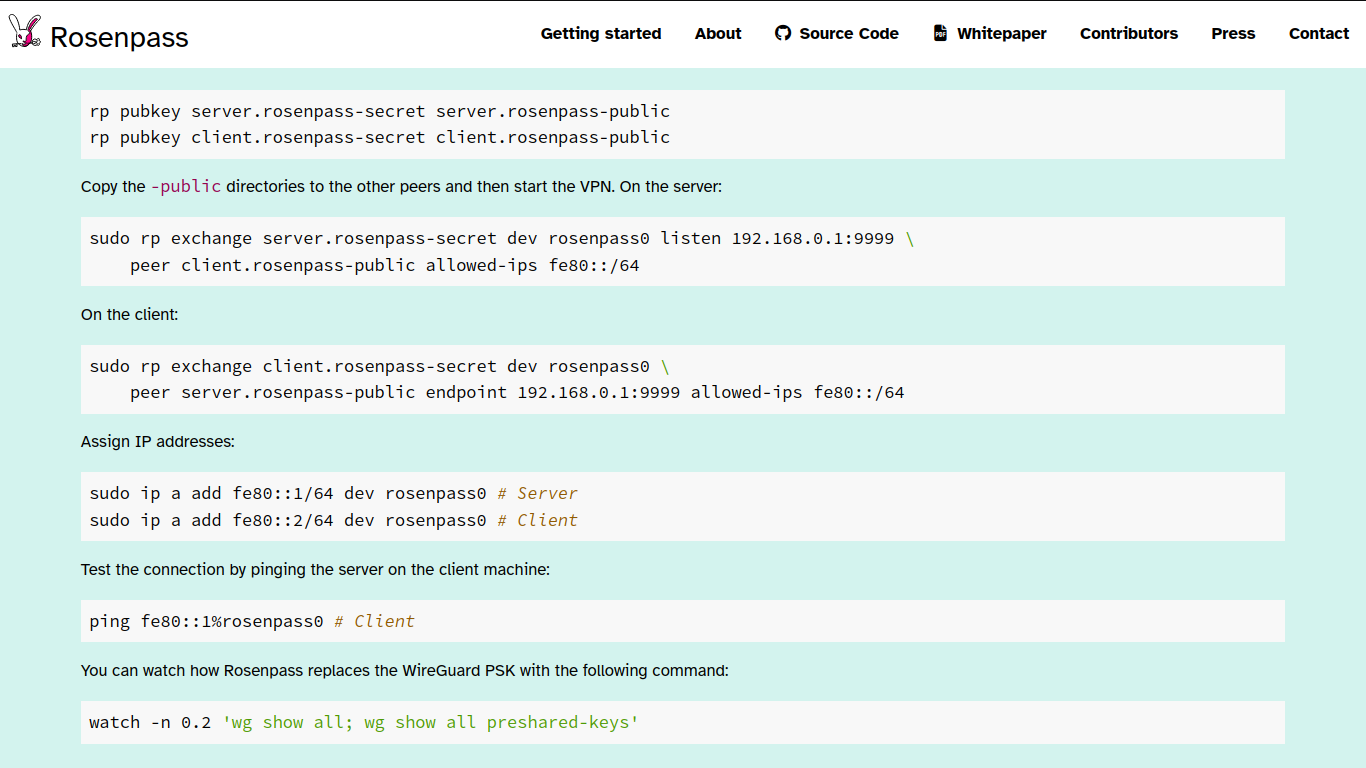
\includegraphics[height=.9\textheight]{assets/2023-03-20-rg-tutorial-screenshot.png}
\end{frame}


\end{document}
